\section{Аналитический раздел}
В этом разделе будет произведен анализ предметной области: описаны основные понятия в области удаления шумов из цветных изображений.
Будут рассмотрены существующие методы удаления импульсных шумов из цветных изображений, приведены результаты сравнительного анализа.
Будет определено понятия нейронной сети, разобран принцип работы сверточной нейронной сети.
Будет сформирована цель работы, постановка задачи формализована в виде IDEF0-диаграммы.

\subsection{Анализ предметной области}
Шум -- дефект изображения, в основе которого лежит эффект появления на фотографии пикселей случайного цвета на изображении \cite{shum}. 

Причины возникновения такого эффекта делятся на два типа: естественные и искусственные.
Основных источником естественных помех на изображениях является фотосенсор \cite{shum}.
Существует несколько физических объяснений появления шума на изображении \cite{causes}:
\begin{enumerate}
	\item При дефектах потенциального барьера происходит утечка заряда. В этом случае шум на изображениях проявляется в виде темных точек на светлом фоне.
	\item При подаче потенциала на электрод может возникнуть темновой ток, который отображается на картинке в виде светлых точек на темном фоне. Основная причина возникновения темнового тока — это примеси в кремниевой пластине или повреждение кристаллической решетки кремния. 
\end{enumerate}

Также шум на изображениях может быть вызван умышленным вмешательством человека или состязательной атакой \cite{impact}. 
Состязательная атака – это манипуляция обучающими данными, архитектурой модели или манипулирование тестовыми данными таким
образом, что это приведет к неправильному выходу из модели машинного обучения \cite{impact}.


Существует несколько основных типов естественных шумов, возникающих на фотографиях \cite{filterTechincs}.
От точного определения характеристики шума зависит то, какой метод требуется выбрать для автоматического определения дефектных пикселей на изображении и последующего его устранения.
Для выявления причины требуется понять, на каком устройстве была сделана фотография, и через какие этапы обработки она прошла.
При этом для реальных цветных фотографий результирующий шум является комбинацией всех возможных типов дефектов, соответственно, нельзя точно сказать о происхождении каждого дефекта на рассматриваемой фотографии \cite{mix}.

\subsubsection{Гауссов шум}
Так как квантовым процессам свойственна случайность, то такие процессы можно отнести к Гауссовым, следовательно, они обладают следующим свойством: распределение суммы независимых случайных величин сходится к нормальному, вне зависимости от характера распределения слагаемых \cite{inproceedings}.

Пусть $I$ -- интенсивность изначального пикселя, а $\nu$ -- интенсивность шума, распределенная по нормальному распределению. 
Тогда интенсивность загрязненного пикселя можно представить по формуле \ref{gauss}: 
\begin{equation}
	\label{gauss}
	I_f = I + \nu,  \nu \sim N(0, \sigma^2).
\end{equation}


Вид гауссова шума представлен на рисунке \ref{fig::gaussSh}:
\FloatBarrier
\begin{figure}[h]	
	\begin{center}
		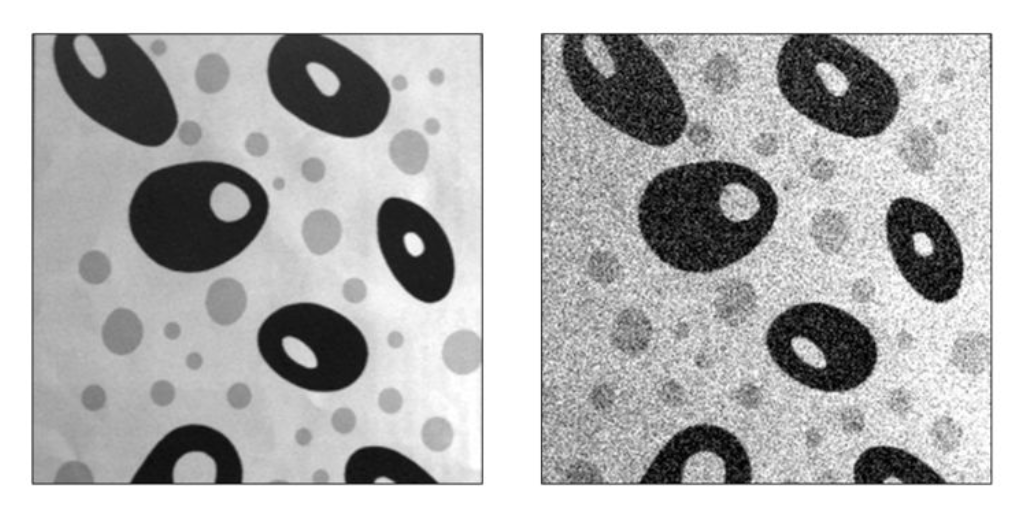
\includegraphics[width=\linewidth]{inc/png/gaussShum.png}
	\end{center}
	\captionsetup{justification=centering}
	\caption{Вид гауссова шума}
	\label{fig::gaussSh}
\end{figure}
\FloatBarrier

Причиной возникновения таких шумов как правило является некорректная работа фотосенсора, что часто происходят в условиях ночного освещения или высокой температуры.
Именно этот вид шумов на практике встречается чаще всего \cite{filterTechincs}. 

\subsubsection{Импульсный шум}
Импульсный шум проявляется в том, что на изображениях в случайных местах появляются черные и белые пиксели \cite{moments}.
Основной причиной их возникновения является темновой ток и утечка заряда в фотосенсоре, а также наличие пикселей с дефектами \cite{shum}.

Когда пиксель имеет белый цвет на темном фоне, то говорят, что здесь присутствует шум соли.
Шум перца -- обратная ситуация: на светлом изображении заметны темные точки \cite{moments}.

Описать появление шума можно по формуле \ref{saltProbe}: 
\begin{equation}
	\label{saltProbe}
	P(S_{i, j} = 1) = p,
\end{equation}
где $S$ -- исходное изображение, $i, j$ -- координаты пикселя, $p$ -- вероятность появления шума. 

Вероятность появления шума зависит от характеристик фотоаппарата, а также от внешних условий, поэтому точно рассчитать значение невозможно \cite{moments}.

\newpage
Вид шума соли и перца представлен на рисунке \ref{fig::salt}:
\FloatBarrier
\begin{figure}[h]	
	\begin{center}
		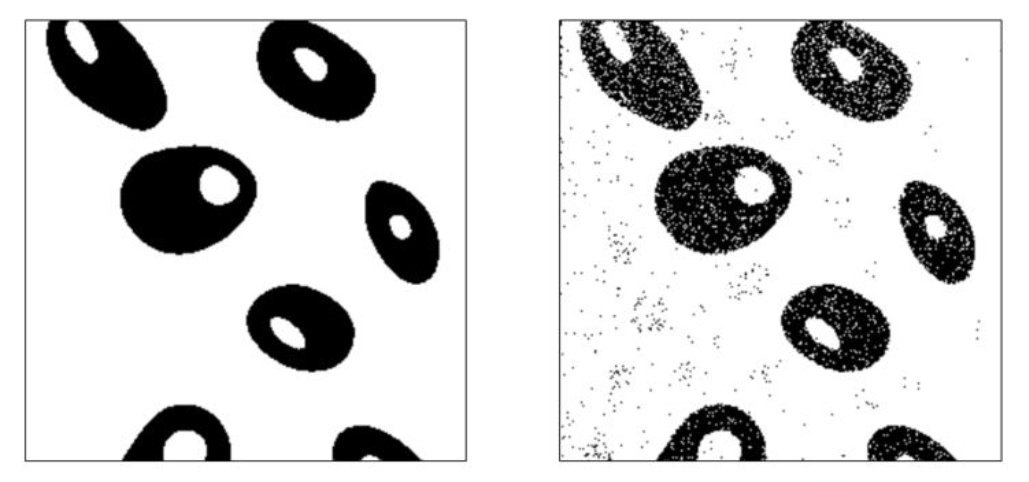
\includegraphics[width=\linewidth]{inc/png/salt.png}
	\end{center}
	\captionsetup{justification=centering}
	\caption{Шум соли и перца}
	\label{fig::salt}
\end{figure}
\FloatBarrier

Основными методами борьбы с таким видом шумов на изображениях являются медианный фильтр и сверточные нейронные сети.

\subsection{Нейронные сети}
Нейронная сеть -- математическая модель, основанная на принципах функционирования биологических нейронных сетей -- например, нервных клеток человека \cite{neural}.
Требуется ввести следующие основные определения в математическом контексте нейронной сети:
\begin{enumerate}
	\item \textbf{Нейрон} -- вычислительная единица, получающая на вход информацию, обрабатывает ее, и возвращает результат на выходе \cite{neural}.
	\item \textbf{Синапс} -- связь между двумя нейронами, построенная по следующему принципу: выход одного нейрона является входом для другого нейрона. 
	У каждого синапса есть один параметр -- вес, который влияет на результат вычислений в нейроне.
	\item \textbf{Слой} -- множество нейронов, которые получают на вход информацию от всех нейронов из предыдущего слоя \cite{neural}.
\end{enumerate}

Все нейроны можно разделить на три больших типа:
\begin{enumerate}
	\item \textbf{Входной} -- он получает на вход исходный вектор, которую требуется обработать в нейронной сети, и без предварительной обработки передаёт на вход следующему слою \cite{ridnet}.
	Графически принято обозначать входной нейрон синим цветом.
	\item \textbf{Выходной} -- значение, полученное на выходе нейрона, считается итоговым результатом всех вычислений нейронной сети \cite{ridnet}.
	На схемах для обозначения выходного нейрона используется зеленый цвет.
	\item \textbf{Скрытый} -- нейрон, который не является ни входным, ни выходным, соответственно, ему на вход поступает информация от других нейронов, и его выход также переходит другим нейронам.
	Скрытые нейроны являются основным вычислительным центром всей сети.
	Выделяются красным цветом.
\end{enumerate}

Математическая модель одного нейрона представляется формулой \ref{matmodel::neiron}:
\begin{equation}
	\label{matmodel::neiron}
	Y = f(\sum_{i = 1}^{N} w_i * x_i + w_0 * x_0),
\end{equation}
где $Y$ -- выход нейрона, $x_i$ -- выход i-го нейрона предыдущего слоя, $w_i$ -- вес синапса, связывающего $x_i$ нейрон и текущий, $x_0$ и $w_0$ -- дополнительный вход и его вес, которые используются для инициализации нейронной сети, $f$ -- передаточная функция.

Пусть $x$ -- значение из входного вектора, $y$ -- результат вычислений нейрона.
На эти значения накладываются ограничения, указанные в формуле \ref{con::neiron}:
\begin{equation}
	\label{con::neiron}
	x \in [0, 1]; y \in [0, 1].
\end{equation}

Передаточная функция является основным параметром нейронной сети.
Как правило, она обладает следующими ключевыми свойствами:
\begin{enumerate}
	\item Передаточная функция $f$ монотонно возрастает.
	\item Область значений функции $f$ лежит в интервале [0, 1].
\end{enumerate}

Передаточная функция позволяет добавлять нелинейность нейронной сети.
Существует несколько основных типов передаточных функций, используемых в нейронных сетях:
\begin{enumerate}
	\item \textbf{Линейная передаточная функция}
	
	В этом случае информация на выходе линейно зависит от результата суммирования входных сигналов.
	В основном она используется для входного слоя нейронной сети, причём коэффициент равен 1.
	
	\item \textbf{Шаговая передаточная функция}
	Алгоритм работы этой функции представлен на формуле \ref{step::neiron}:
	\begin{equation}
		\label{step::neiron}
		f(x)= 
		\begin{cases}
			1,& \text{если } x \geq 1, \\
			0,& \text{если } x \leq 0, \\
			x, & \text{иначе.}
		\end{cases}
	\end{equation}

	Самая распространенная вариация функции -- исправленная линейная передаточная функция или \textbf{ReLu} \cite{relu}.
	Математически она описывается формулой \ref{relu::neiron}:
	\begin{equation}
		\label{relu::neiron}
				f(x)= 
		\begin{cases}
			x,& \text{если } x \geq 0, \\
			0,& \text{иначе.}
		\end{cases}
	\end{equation} 

	Она получила широкое распространение в сверточных нейронных сетях из-за простоты использования \cite{CNN_translate}.
	
	\item \textbf{Сигмоидальная передаточная функция}
	
	Эта передаточная функция позволяет усиливать слабые сигналы значительно заметнее, чем сильные, поэтому область сильных сигналов представлена пологими участками \cite{relu}.
	
	На формуле \ref{sigmoid::neiron} представлен вид передаточной функции \cite{CNN_translate}:
	
	\begin{equation}
		\label{sigmoid::neiron}
		f(x) = \frac{1}{1 + \exp(-tx)},
	\end{equation}
	где $t$ -- параметр функции, регулирующий крутизну функции.
	
	\item \textbf{Гиперболическая передаточная функция}
	Эта передаточная функция использует операцию гиперболического тангенса для расчёта итогового значения \cite{relu}.
	По свойствам она похожа на сигмоиду, но слабые сигналы усиливаются еще сильнее.
	
	Формула гиперболической передаточной функции \ref{hyper::neiron}:
	\begin{equation}
		\label{hyper::neiron}
		f(x) = \frac{2}{1 + \exp(-2x)} + 1.
	\end{equation}
\end{enumerate}

Перед тем, как нейросеть начнет вычислять результат, требуется провести ее обучение.

Для этого используется метод обратного распространения ошибки.

Предположим, для заданного сигнала заранее известен вектор результатов $Y0$, который ожидается на выходе нейронной сети.
Нейронная сеть после подачи на вход сигнала выдала вектор $Y1$.

Функция ошибки для отдельного синапса, полученная методом наименьших квадратов, представлена на формуле \ref{error::neiron}:
\begin{equation}
	\label{error::neiron}
	E{w} = \frac{1}{2} * \sum{N}{i = 0} (Y0_i - Y1_i)^2.
\end{equation}

Для проведения обучения нейронной сети используется стохастический градиентный спуск. 
Требуется изменять веса после вычислений результат для каждого входящего нейрона.

Добавленное значение к весу представлено на формуле \ref{delta::neiron}:
\begin{equation}
	\label{delta::neiron}
	\Delta w_{ij} = -\eta * \frac{\partial E}{\partial w_{ij}},
\end{equation}
где $w_{ij}$ -- вес синапса между нейронами $i$ и $j$, $\eta$ -- коэффициент, влияющий на скорость обучения.

Суть обучения нейронной сети состоит в минимизации функции ошибки для отдельного входящего сигнала.
С помощью корректировки коэффициентов синапсов сеть пытается достигнуть точки сходимости или локального минимума.
Именно для этого используется градентный спуск.

\subsubsection{Сверточная нейронная сеть}
Сверточная нейронная сеть -- один из подвидов нейронных сетей, получивший широкое распространение в области обработки изображений \cite{CNN_research}.

В контексте СНС нужно ввести следующие определения:
\begin{enumerate}
	\item \textbf{Ядро свертки} -- квадратная матрица весов, используемая для операции свертки \cite{CNN_2}. 
	Ее размер, как правило, определяется программистом при инициализации сети.
	\item \textbf{Свертка} -- математическая операция, в результате которой уменьшается размерность вектора исходного сигнала \cite{CNN_arch}.
	Ее можно описать следующей формулой \ref{conv::neiron}:
	\begin{equation}
	  	\label{conv::neiron}
	  	x_{i}^{l} = f(\sum{}{i} x_{i}^{l-1} * k_{j}^{l} + b_{j}^{l}),
	\end{equation}
	где $x_{i}^{l}$ -- выходной сигнал слоя $l$, $f$ -- передаточная функция, $x_{i}^{l-1}$ -- входной сигнал для входа $l$,
	$k_{j}^{l}$ -- ядро свертки слоя $l$, $b_{j}^{l}$ -- коэффициент сдвига для слоя $l$.
	
	\item \textbf{Карта признаков} -- результат, полученный после операции свертки, который отражает наличие какого-либо признака во входном сигнале \cite{CNN_arch}.
\end{enumerate}

Процесс обучения сверточной нейронной сети осуществляется методом обратного распространения ошибки \cite{CNN_arch}.
В сверточной нейронной сети несколько ядер свертки, которые отвечают за отдельные признаки, но такое разбиение возникает в результате обучения -- программист не предусматривает это при проектировании архитектуры сети.
Таким образом, каждый набор вес весов формирует собственную карту признаков, в результате возникает явление многоканальности в нейронной сети: на одном слое появляются независимые карты признаков \cite{CNN_pool}. 
Во время выполнения операции свертки ядро матрицы передвигают не на полный шаг, а на маленькое расстояние -- несколько пикселей, в результате искомый признак отражается в нескольких весах выходного вектора.

Так как в результате свертки итоговая размерность векторов уменьшается, то величина сигнала стремится к размерам ядра свертки.
Последовательность таких действий называется \textit{субдискретизацией} \cite{CNN_pool}.

В качестве передаточной функции чаще всего используют ReLu \cite{CNN_pool}.

Архитектура сверточной сети состоит из нескольких компонентов:
\begin{enumerate}
	\item \textbf{Начальный слой} -- принимает на вход исходное изображение \cite{CNN_research}.
	\item \textbf{Сверточные слои} -- состоят из ядр свертки, каждый слой выполняют субдискретизацию полученных карт признаков \cite{CNN_research}.
	\item После прохождения субдискретизации карты признаков вырождаются до векторов или скаляров. 
	В дальнейшем они попадают на нейроны из полносвязной нейронной сети, которая рассчитывает итоговый результат.
\end{enumerate}

При прохождении через сверточные слои размерность каждого слоя уменьшается, в то время как количество каналов -- растет.
Это позволяет использовать полносвязную нейронную сеть для определение результата \cite{CNN_arch}.

Схематично архитектура сверточной нейронной сети представлена на рисунке \ref{analit::CNN}:
\FloatBarrier
\begin{figure}[h]	
	\begin{center}
		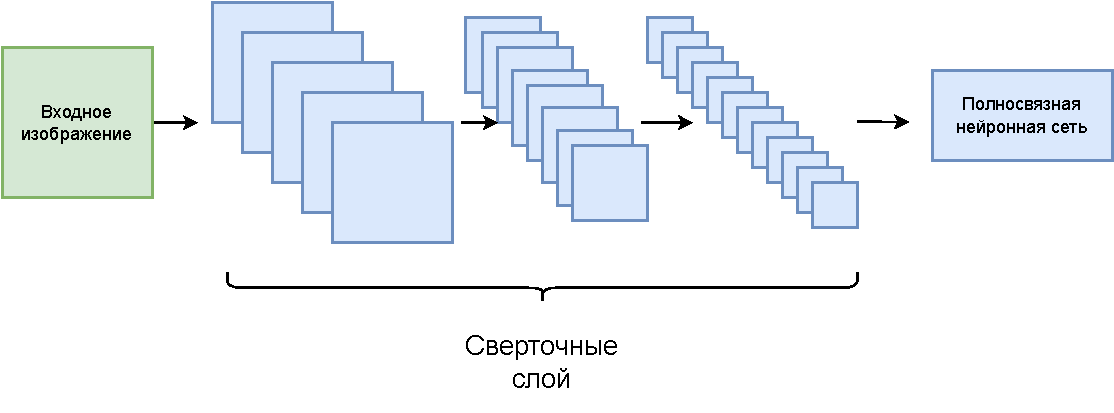
\includegraphics[width=\linewidth]{inc/pdf/CNN.pdf}
	\end{center}
	\captionsetup{justification=centering}
	\caption{Архитектура сверточной нейронной сети}
	\label{analit::CNN}
\end{figure}
\FloatBarrier

Во время обучения принято на некоторых итерациях убирать из сети одиночные нейроны, что позволяет точнее настроить другие нейроны для более точного обучения \cite{ridnet}.

Признакам, сформированные в результате работы нейронной сети, невозможно дать объяснение, поэтому в случае, если нейронная сеть перестает выполнять поставленную задачу, разработчики изменяют ее конфигурацию или выбирают другой этап применения в общем алгоритме \cite{CNN_2}. 

На текущий момент не существует архитуктур нейросетей, которые бы в точности позволяли бороться с шумами в изображениях, поэтому подходящие настройки сети подбираются экспериментально \cite{neural}.

Нейронные сети активно применяются в области удаления шумов из изображений, так как они позволяют распознать и удалить шумы, с которыми не справляются стандартные методы.
Для трехмерных изображений ядра матрицы составляются для каждого из составляющих цветов пикселя, итоговые результаты по цветам суммируется \cite{ridnet}. 
Это позволяет менять вариативность нейронной сети, например, настраивать на более приоритетный цвет.

\subsection{Обзор существующих методов}
Шумы искажают исходную картинку и портят ее качество так, что это способен распознать человеческий глаз.
Однако могут возникнуть трудности в обнаружении помех, поскольку они трудно различимы при совпадении цвета фона и цвета пикселя, например, светлые точки будут плохо заметны на ярком фоне.

Было разработано несколько алгоритмов, которые производят бинарную классификацию пикселей и определяют, какие из них можно идентифицировать как шумы и затем их устранить.

В качестве классификации алгоритмы можно разделить на два типа:
\begin{enumerate}
	\item \textbf{Изотропная фильтрация} -- такие методы устраняют помехи, но не учитывают детали пикселя и увеличивают размытость.
	\item \textbf{Анизотропная фильтрация} -- алгоритмы устраняют эффекты сглаживания, уменьшают размытость и сохраняют детали пикселя, устраняя при этом непосредственно шум из изображения.
\end{enumerate}


\subsection{Общий алгоритм работы фильтров}
Алгоритмы, анализирующие наличие шумов в изображениях, имеют дело с различными характеристиками одного пикселя.
Например, цвет пикселя можно разбить на три составляющие -- синюю, красную и зеленую \cite{color}. 

В таком случае метод работает с каждой из составляющих пикселя, вычисляя новое значение для каждой характеристики.
Результат работы в этом случае является объединением подсчетов по всем характеристикам.

Общая схема работы алгоритмов представлена на рисунке \ref{fig::allAlgs}:
\FloatBarrier
\begin{figure}[h]	
	\begin{center}
		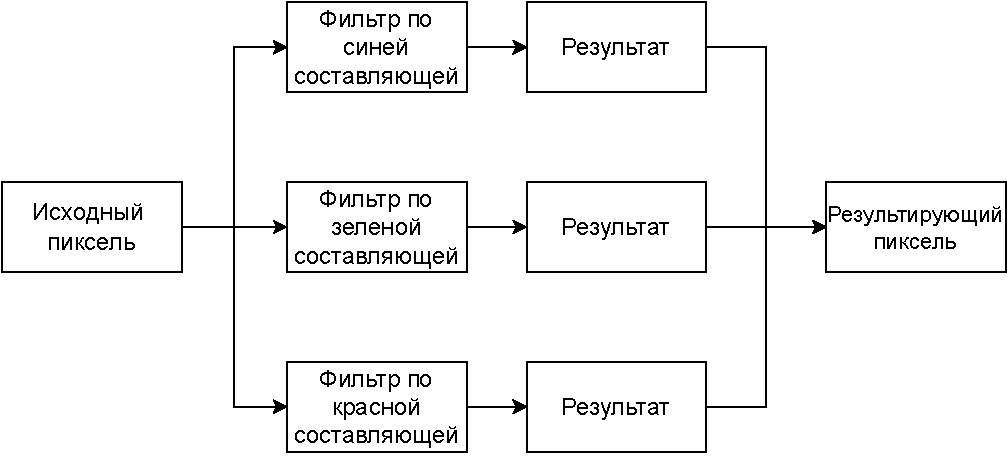
\includegraphics[width=\linewidth]{inc/pdf/allAlgs.pdf}
	\end{center}
	\captionsetup{justification=centering}
	\caption{Общая схема работы всех алгоритмов}
	\label{fig::allAlgs}
\end{figure}
\FloatBarrier

Каждый из фильтров, перечисленный ниже, работает с каждым из параметров пикселя одинаково, поэтому для корректной работы алгоритмов требуется вычислить значение каждого свойства для результирующего пикселя \cite{filterTechincs}.

\newpage
\subsubsection{Медианный фильтр}
Под медианным фильтром понимается семейство однотипных алгоритмов, относящихся к классу нелинейных фильтров \cite{median}.

Метод работает в цикле с каждым пикселем изображения \cite{filterTechincs}. 
В окрестности каждого пикселя находится восемь соседних, каждый обладает собственными свойствами. 

На рисунке \ref{fig::grid} изображена сетка, с которой работает алгоритм:

\FloatBarrier
\begin{figure}[h]	
	\begin{center}
		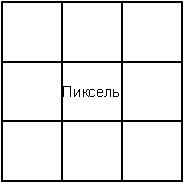
\includegraphics[]{inc/pdf/grid.pdf}
	\end{center}
	\captionsetup{justification=centering}
	\caption{Рассматриваемая сетка пикселей при работе алгоритма}
	\label{fig::grid}
\end{figure}
\FloatBarrier

Пусть $C_{i, j}$ -- один из параметров рассматриваемого пикселя, а $\Omega$ -- все пиксели сетки.
Алгоритм подсчитывает медиану от такого же параметра соседних клеток и заменяет параметр пикселя на значение этой медианы \cite{median}.

\newpage
Схема работы алгоритма изображена на рисунке \ref{fig::median}:
\FloatBarrier
\begin{figure}[h]	
	\begin{center}
		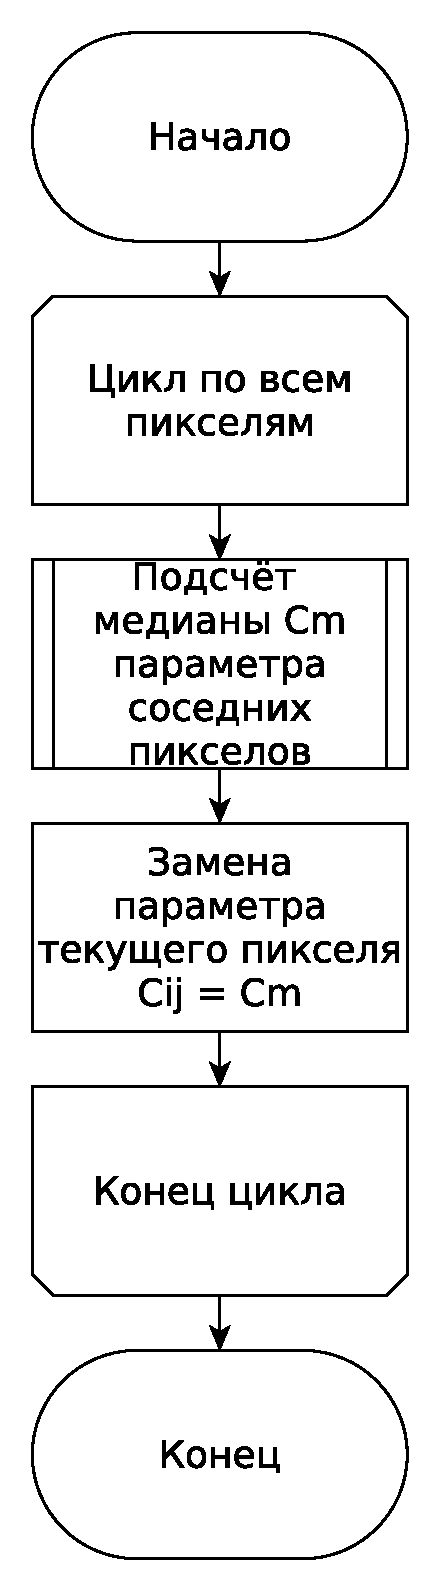
\includegraphics[height=15cm]{inc/pdf/median.pdf}
	\end{center}
	\captionsetup{justification=centering}
	\caption{Схема работы алгоритма медианного фильтра}
	\label{fig::median}
\end{figure}
\FloatBarrier

К недостаткам данного метода можно отнести то, что алгоритм может убрать значительные детали из изображения, посчитав их за шум \cite{median2}. 


\subsubsection{Гауссовский фильтр}
Работа алгоритма гауссовского фильтра также зависит от значений цветовых свойств пикселей в сетке, рассмотренной на рисунке \ref{fig::grid}.

В этом случае для каждого соседнего рассчитывается вес, с которым он влияет на новое значение рассматриваемого пикселя  \cite{filterTechincs}. 
Пусть $d$ -- расстояние до центрального пикселя сетки, $\sigma$ -- стандартное отклонение, подсчитанное для всех значений определенного параметра текущей сетки.
Тогда вес $w$ пикселя рассчитывается по формуле \ref{weight}:
\begin{equation}
	\label{weight}
	w_{ij} = e^{\left(\frac{-d^2}{2\sigma^2}\right)}.
\end{equation}

Подсчитав вес для каждого пикселя в сетки, можно рассчитать новое значение свойства рассматриваемого пикселя по формуле \ref{gauss::final}:
\begin{equation}
	\label{gauss::final}
	p_i = \frac{1}{\sum_{j \in \Omega}^{} w_{ij}} * \sum_{j \in \Omega}^{} w_{ij} * p_j.
\end{equation}

Схема алгоритма гауссовского фильтра представлена на рисунке \ref{fig::gauss}:
\FloatBarrier
\begin{figure}[h]	
	\begin{center}
		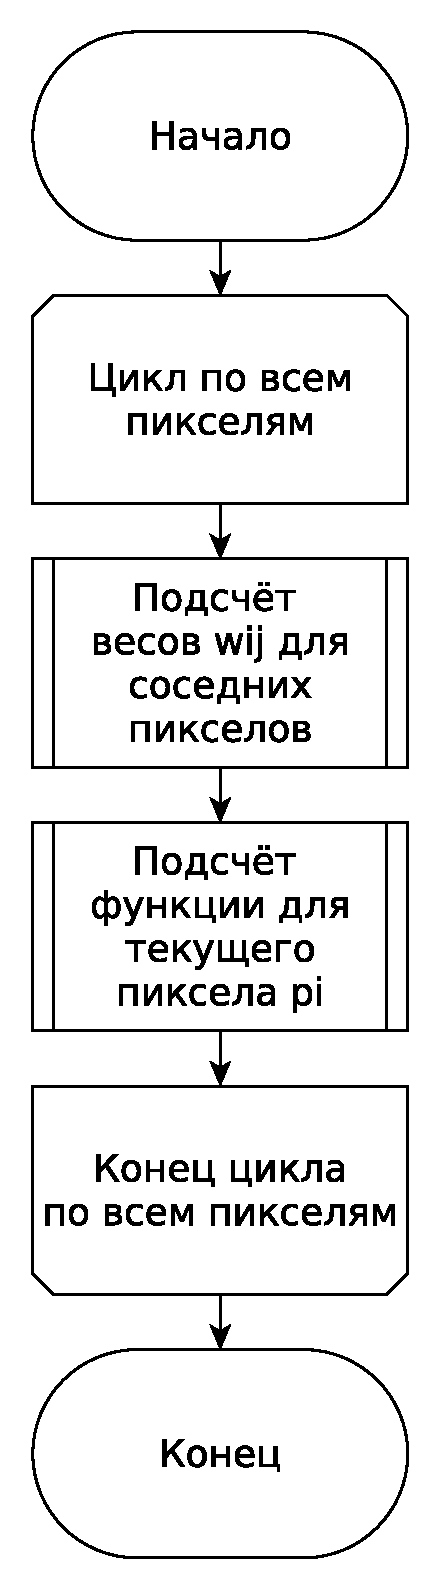
\includegraphics[height=10cm]{inc/pdf/gauss.pdf}
	\end{center}
	\captionsetup{justification=centering}
	\caption{Схема работы алгоритма гауссовского фильтра}
	\label{fig::gauss}
\end{figure}
\FloatBarrier

\subsubsection{Билатеральный фильтр}
Алгоритм билатеральной фильтрации является улучшением метода Гауссовского фильтра \cite{bilateral}.

Для каждого пикселя сетки соседних пикселей используется сразу два веса: один аналогичный параметру из исходного алгоритма, а второй отвечает за анизотропную составляющую. 

Расчет веса $w_s$, отвечающего за изотропную составляющую, происходит по формуле \ref{weight}. 
Коэффициент, регулирующий анизотропные свойства фильтрации, рассчитывается по формуле \ref{weight2}:
\begin{equation}
	\label{weight2}
	w_{r} = \exp\left(\frac{-|p_i - p_j|}{2\sigma^2}\right).
\end{equation}

В таком случае результат работы некоторого пикселя можно посчитать по формуле \ref{bilateral}:
\begin{equation}
	\label{bilateral}
	p_i = \frac{1}{\sum_{j \in \Omega}^{} w_{s}w_{r}} * \sum_{j \in \Omega}^{} w_{s}w_{r}p_j.
\end{equation}

Схема работы алгоритма представлена на рисунке \ref{fig::bilateral}:
\FloatBarrier
\begin{figure}[h]	
	\begin{center}
		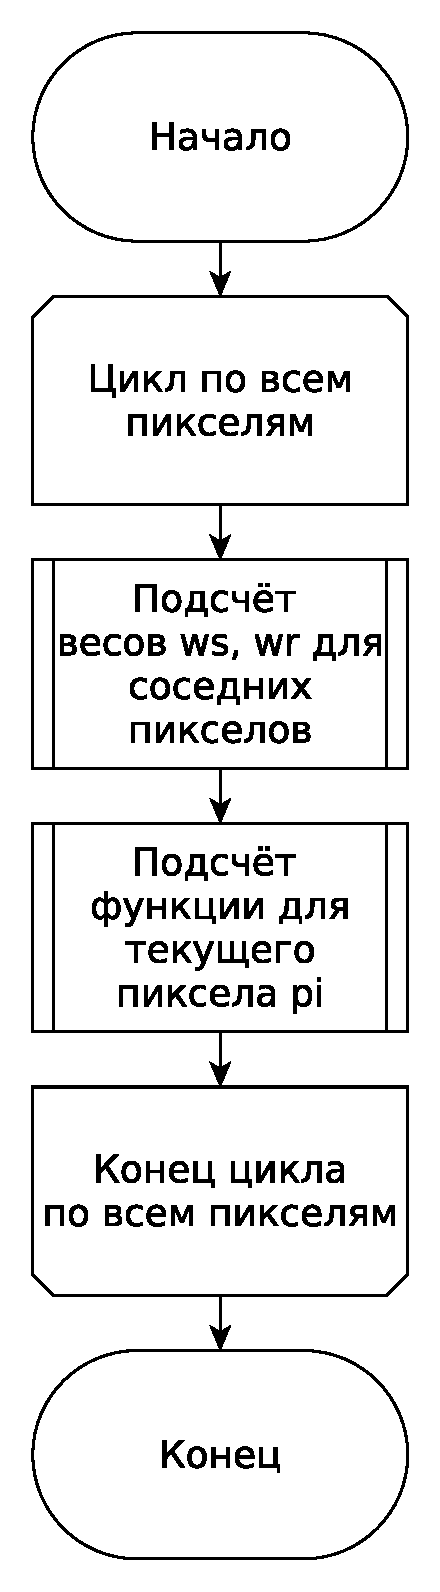
\includegraphics[height=10cm]{inc/pdf/bilateral.pdf}
	\end{center}
	\captionsetup{justification=centering}
	\caption{Схема работы алгоритма билатеральной фильтрации}
	\label{fig::bilateral}
\end{figure}
\FloatBarrier

\subsubsection{Алгоритм Цзяньвэй}
Этот алгоритм был описан в 2014 году индонезийским ученым Ван Цзяньвэй \cite{color_image}.
Алгоритм позволяет эффективно убирать шумы соли и перца даже в случае сильной загрязненности изображения.

Процедура заключается в обходе всех пикселей фотографии в заданном порядке и определении того, соответствуют ли значения пикселей функции плотности вероятности импульсного шума или нет. 
Если пиксель на первом классифицируется как шум, то подсчитывается количество импульсного шума в маске определенной формы.
Результатом операции маски является замена значения пикселя.
В противном случае это не рассматривается как шум, значение пикселя остается неизменным.

Схема алгоритма Цзяньвэй представлена на рисунке \ref{fig::china}:
\FloatBarrier
\begin{figure}[h]	
	\begin{center}
		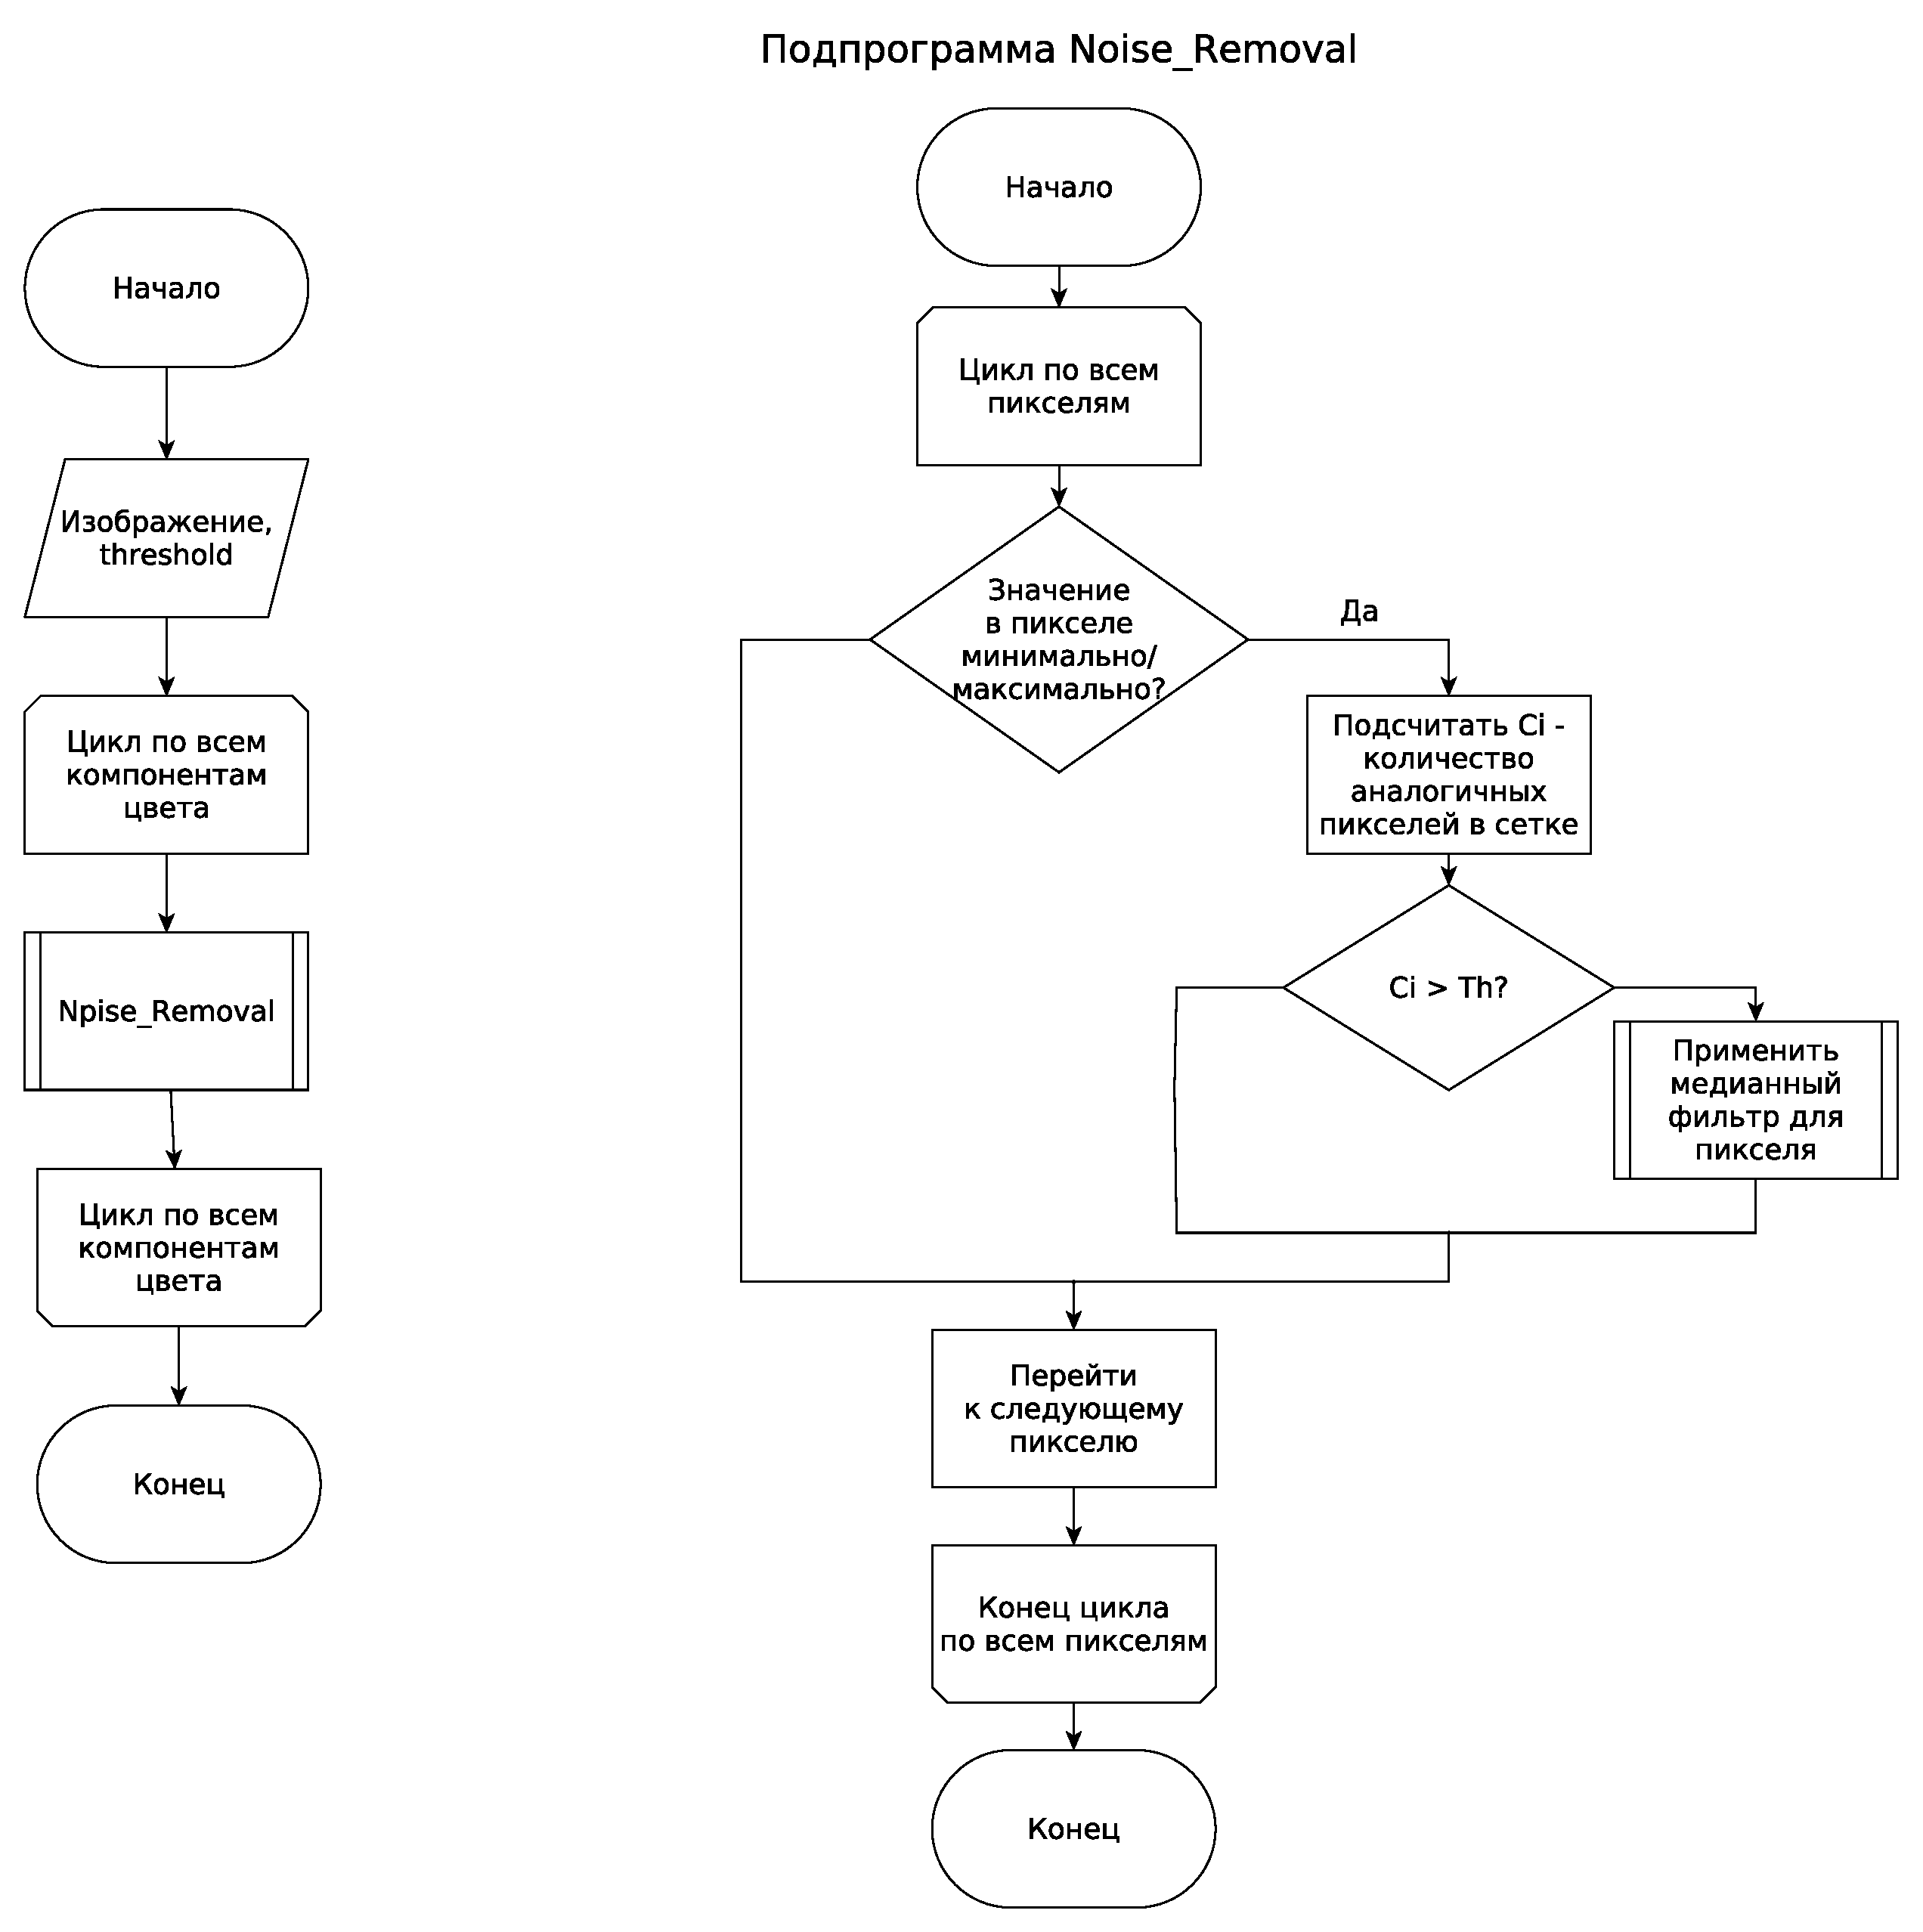
\includegraphics[height=13cm]{inc/pdf/china.pdf}
	\end{center}
	\captionsetup{justification=centering}
	\caption{Схема работы алгоритма Цзяньвэй}
	\label{fig::china}
\end{figure}
\FloatBarrier

\subsubsection{DnCNN}
Алгоритмы, основанные на сверточных нейронных сетях, получили широкое распространение в области удаления шумов из изображений.
Они применяются в ситуациях, требующих восстановления исходного изображения по имеющемуся загрязненному фото, например, при анализе снимков из телескопов или фотоаппаратов \cite{neural}. 
DnCNN относится к этому классу методов.

Перед запуском алгоритма требуется задать суммарную глубину слоев $D$, а также количество цветовых составляющих $c$ -- для цветных изображений $c=3$, для серых $c=1$ \cite{dcnn}. Всего в конфигурации нейронной сети используется три типа слоев \cite{dcnn2}:
\begin{enumerate}
	\item Первый слой состоит из 64 фильтров размером $3*3*c$, в качестве функции активации используется ReLU.
	\item Следующие $2*(D - 1)$ слоев состоят из фильтров размером $3*3*64$, между каждым слоем применяется пакетная нормализация.
	\item Последний слой состоит из $c$ фильтров размером $3*3*64$ каждый.
\end{enumerate}

Во всех слоях, кроме последнего, используется ReLU в качестве функции активации нейрона \cite{dcnn}. 

Пусть $x$ -- входное значение нейрона. 

Тогда выход считается по формуле \ref{dncnn}: 
\begin{equation}
	\label{dncnn}
	f(x) = \mathrm{max}(0, x).
\end{equation}

Конфигурация нейронной сети представлена на рисунке \ref{fig::dncnn}:
\FloatBarrier
\begin{figure}[h]	
	\begin{center}
		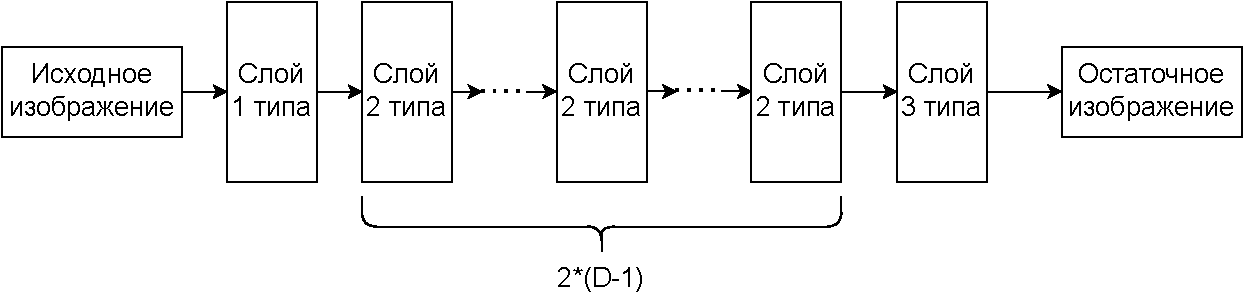
\includegraphics[width=\linewidth]{inc/pdf/dnn.pdf}
	\end{center}
	\captionsetup{justification=centering}
	\caption{Конфигурация нейронной сети в алгоритме DNCNN}
	\label{fig::dncnn}
\end{figure}
\FloatBarrier

\newpage
На выходе алгоритма получается остаточное изображение $R$. 
Пусть $Y$ -- исходное изображение.
Тогда очищенный снимок $X$ можно посчитать по формуле \ref{dncnnres}:
\begin{equation}
	\label{dncnnres}
	X = Y - R.
\end{equation}

\subsubsection{RIDNet}
Алгоритм RIDNet также использует сверточные нейронные сети, однако в его основе лежит другой подход \cite{ridnet2}.
Идея состоит в том, что не во всех ситуациях требуется, чтобы модель одинаково оценивала каждую цветовую составляющую пикселя, поэтому у каждой из составляющих будет свой вес \cite{ridnet}.

Конфигурация сети состоит из трех основных модулей \cite{ridnet}: 
\begin{enumerate}
	\item \textbf{Модуль извлечения признаков} -- он состоит из одного слоя, который производит свертку изображения и инициализирует  признаки $f_0$.
	\item \textbf{Модуль извлечения остаточных признаков из остаточного изображения} -- выполняет основную работу в сети, состоит из четырех дополнительных модулей -- EAM (Enhancing attention module).
	\item  \textbf{Модуль реконструкции изображения} -- использует один слой, восстанавливает исходное изображение. ReLU используется в качестве передаточной функции.
\end{enumerate}

При этом модули в алгоритме связаны между собой, например, после прохождения первого модуля полученный результат попадает на вход как второго модуля, так и третьего.

Общая конфигурация нейронной сети представлена на рисунке \ref{fig::ridnetall}:
\FloatBarrier
\begin{figure}[h]	
	\begin{center}
		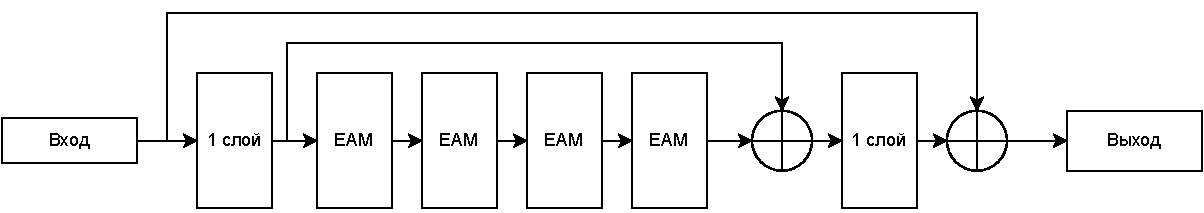
\includegraphics[width=\linewidth]{inc/pdf/ridnet.pdf}
	\end{center}
	\captionsetup{justification=centering}
	\caption{Обшая конфигурация нейронной сети в алгоритме RIDNet}
	\label{fig::ridnetall}
\end{figure}
\FloatBarrier

EAM внутри себя состоит из множества различных слоев, которые комбинируются между собой \cite{ridnet}.
Каждый модуль внутри себя выполняет три действия: выделяет основные признаки из изображения, сжимает изображение для большей производительности и увеличивает веса по наиболее значимым признакам.

Внутри модуля используются сетки размером $3x3$. 
В качестве функции активации на выходе последнего слоя EAM используется сигмоида. 
Пусть $x$ -- вход нейрона, тогда выход можно посчитать по формуле \ref{sigm}:
\begin{equation}
	\label{sigm}
	f(x) = \frac{1}{1+e^x}.
\end{equation}

При этом авторы алгоритма предложили использовать больше, чем четыре EAM-модуля, однако это не увеличило результаты работы алгоритма \cite{ridnet2}.
Также в алгоритме предусмотрено использование регуляризации для борьбы с переобучением системы.

\subsection{Критерии сравнения алгоритмов}
Для верификации работы алгоритмов используются открытые наборы реальных изображений. 
Алгоритмам предоставляют на вход загрязненные изображения, в результате получается очищенное изображение.
У начальных изображений зафиксирован одинаковый размер, так как это позволяет зафиксировать размер входа для нейронной сети.
Для полученного результата подсчитываются метрики, и на их основе устанавливается эффективность для метода.

Для сравнения результатов используется две основные метрики: PSNR и SSIM \cite{vs}.

\subsubsection{PSNR}
PSNR -- метрика, обозначающее пиковое отношение сигнала к шуму \cite{rs}.
Она универсальна и используется не только для удаления шумов, а также для измерения уровня искажения при сжатии изображений.
PSNR рассчитывается по логарифмической шкале.

Пусть есть два изображения $I$ -- исходное, и $K$ -- полученное в результате обработки.
Размер каждого составляет $MxN$ пикселей.

Разница между ними рассчитывается по формуле \ref{mse} \cite{rs}:
\begin{equation}
	\label{mse}
	\mathrm{MSE} = \frac{1}{MN}\sum_{0}^{M-1}\sum_{0}^{N-1}|I(i, j) - K(i, j)|.
\end{equation}

Максимальное значение любого пикселя обозначим за MX. 
Чаще всего оно равно 255 \cite{rs}.
Теперь искомую метрику PSNR можно рассчитать по формуле \ref{PSNR}:
\begin{equation}
	\label{PSNR}
	\mathrm{PSNR} = 20\log_{10}\left(\frac{\mathrm{MX}}{\sqrt{\mathrm{MSE}}}\right).
\end{equation}

Метрика изначально была создана для монохромных изображений, поэтому для цветных изображений результат усредняется по каждой из цветовых составляющих пикселя.

\subsubsection{SSIM}
SSIM -- метрика, обозначающая индекс структурного сходства изображений \cite{ssim}. 
В отличие от PSNR, эта характеристика позволяет учесть не только разницу в фактических величинах между пикселями, но и взаимосвязь между ними, то есть структурное сходство.

Пусть есть два изображения $I$ -- исходное, и $K$ -- полученное в результате обработки.
Размер каждого составляет $MxN$ пикселей. 
Для каждого изображения были рассчитаны характеристики: $\mu_{i}$ -- среднее по цветовой составляющей для изображения $i$, $\sigma^2_i$ -- дисперсия цветовой составляющей для фотографии $i$, $\sigma_{ij}$ -- ковариация цветовой составляющей для изображений $i$ и $j$. 

Также вводится константа $L$, которая обозначает динамический диапазон. 
Как правило, она равняется 255 \cite{ssim}. 

Исходя из этого, метрику SSIM можно рассчитать по формуле \ref{SSIM}:
\begin{equation}
	\label{SSIM}
	\mathrm{SSIM} = \frac{(2\sigma^2_{I}\sigma^2_{K} + 0.01L)(2\sigma^2_{IK} + 0.03L)} { (\mu^2_{I}+\mu^2_{K} +0.01L)  (\sigma^2_{I} +\sigma^2_{K} +0.03L) }.
\end{equation}

\newpage
\subsection{Классификация существующих решений}
Классификацию существующих алгоритмов можно привести к таблице.
В качестве основных параметров классификации были использованы следующие признаки:
\begin{itemize}
	\item учитывается ли анизотропная составляющая при очистке изображения от шумов;
	\item учитывают ли алгоритмы взаимосвязь пикселей между собой;
	\item используются ли алгоритмом нейронные сети;
	\item происходит ли сглаживание в ходе работы алгоритма;
	\item какой размер изображения требуется для его работы;
	\item для какого вида шумов используется алгоритм.
\end{itemize}

Классификация существующих алгоритмов представлена на таблице \ref{table::class}.
Под заголовком Gauss приведены критерии для алгоритма гауссовского фильтра, под заголовком Median -- для алгоритма медианного фильтра, Bilat -- для билатерального фильтра, Jianwei -- для алгоритма Цзяньвэй.
\FloatBarrier
\begin{table}[h]
	\caption{Таблица сравнения существующих алгоритмов}
	\captionsetup{justification=raggedright,singlelinecheck=false}
	\centering
	\begin{tabular}{ | p{4cm} | p{1.6cm} | p{1.7cm} | p{1.7cm} | p{1.5cm} | p{1.7cm}| p{1.7cm} |}
		\hline
		& Median  & Gauss & Bilat & Jianwei & DnCNN &  RIDNet \\ 
		\hline
		Учитывается ли
		анизотропия?     & нет          & нет	  	 &  да        &	да & да & да \\
		\hline
		Учитывается ли взаимосвязь пикселей?   & нет  & да  	 &  да	   &	да		& нет & да \\
		\hline
		Происходит ли сглаживание? & нет 	& да & да & да & нет &  нет	   \\
		\hline
		C каким шумом работает метод?  & любой & гауссов &  гауссов  & любой & любой & гауссов \\
		\hline
		Используются нейронные сети?  & нет 	& нет 		 &  нет	   &	нет		& да & да \\
		\hline
	\end{tabular}
	\label{table::class}
\end{table}
\newpage

Полученные результаты можно свести к следующим тезисам:
\begin{itemize}
	\item шум на изображениях возникает вследствие несовершенства технических средств. На практике применяются алгоритмические средства борьбы;
	\item существующие алгоритмы, не использующие нейронные сети, справляются лишь с определенным видом шумов, имея проблемы с устранением остальных типов;
	\item в алгоритмах DnCNN и RIDNet детали реализации сети могут быть изменены: функция активации, количество слоев;
	\item новые решения в области удаления шумов являются лишь улучшением или комбинированием уже существующих алгоритмов.
\end{itemize}

\subsection{Формулировка цели}
В ходе выполнения работы требуется разработать метод, позволяющий удалить импульсные шумы из цветных изображений. 
Метод должен отвечать следующим требованиям:
\begin{enumerate}
	\item Должны удаляться импульсные шумы для цветных изображений любого размера.
	\item Гарантируется, что максимальное количество процентов шума -- до 30\% зашумленных пикселей.
	\item Исходное количество шума неизвестно.
	\item Для выполнения цели должны быть использованы нейронные сети.
\end{enumerate}

\newpage
\subsection{Формализация задачи. IDEF0-диаграмма}
Для формализации задачи была составлена IDEF0-диаграмма нулевого и первого уровня. 

IDEF0-диаграмма нулевого уровня представлена на рисунке \ref{idef0::0}:

\FloatBarrier
\begin{figure}[h]	
	\begin{center}
		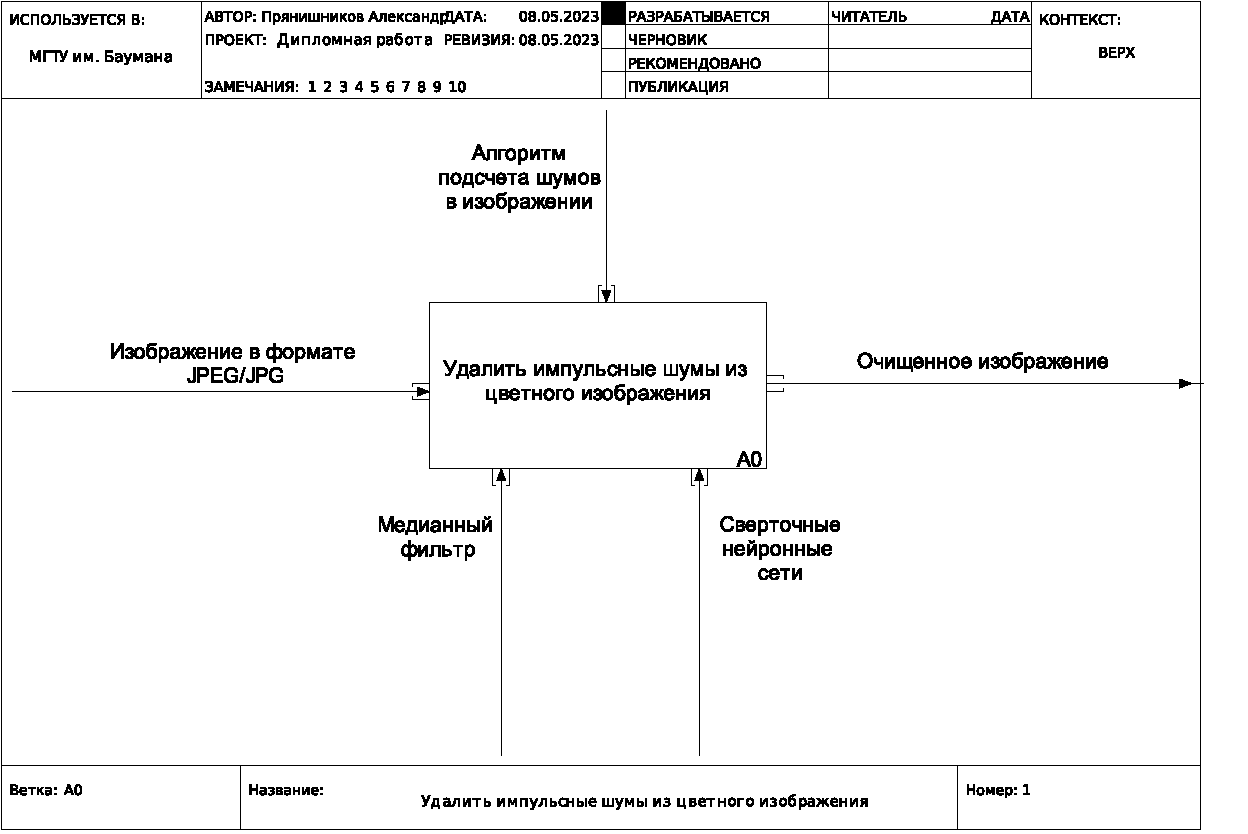
\includegraphics[height=7cm]{inc/pdf/01_A0.pdf}
	\end{center}
	\captionsetup{justification=centering}
	\caption{IDEF0-диаграмма нулевого уровня}
	\label{idef0::0}
\end{figure}
\FloatBarrier

IDEF0-диаграмма первого уровня представлена на рисунке \ref{idef0::1}:

\FloatBarrier
\begin{figure}[h]	
	\begin{center}
		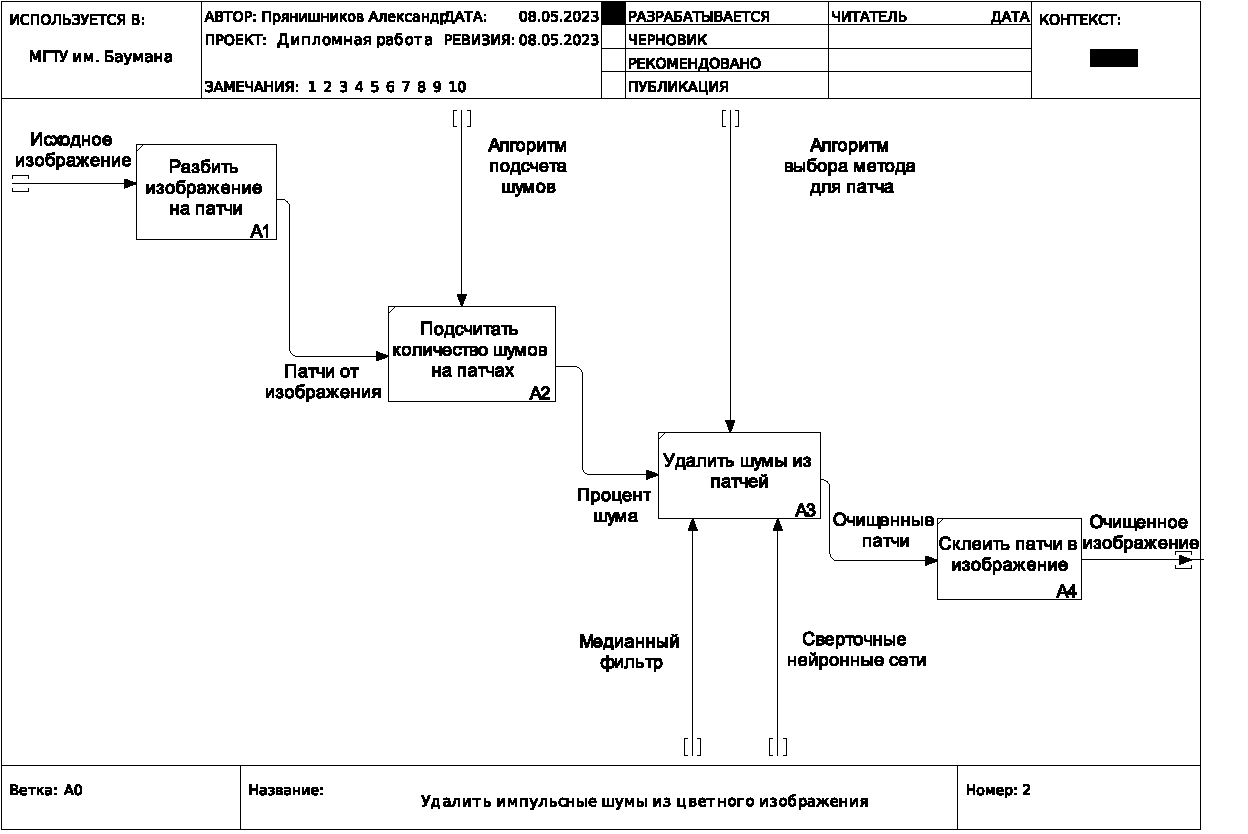
\includegraphics[height=7cm]{inc/pdf/02_A0.pdf}
	\end{center}
	\captionsetup{justification=centering}
	\caption{IDEF0-диаграмма первого уровня}
	\label{idef0::1}
\end{figure}
\FloatBarrier

\subsection*{Выводы}
Был проведен анализ предметной области, введены основные понятия.
Описаны физические причины появления шумов на изображениях.
Разобраны основные алгоритмы, которые используются в области удаления шумов, представлены схема их работы.
Результаты сравнительного анализа представлены в табличном виде.

Была сформирована цель работы.
Задача была формализована в виде IDEF0-диаграммы.